\documentclass{article}
\usepackage{afterpage}
\usepackage{float}
\usepackage{longtable}
\usepackage{graphicx}
\usepackage{pdflscape}
\usepackage[numbers,sort&compress]{natbib}
\usepackage{psfrag}

\usepackage{amsmath}
\usepackage{amsfonts}
\usepackage{graphicx}
%\usepackage{nicefrac}
\usepackage{graphicx}
\usepackage{caption}
% \usepackage{subcaption}
\usepackage{subfigure}
% \usepackage{algorithm}
% \usepackage{paralist}
% % \usepackage[geometry]{ifsym}
\usepackage{rotating}
\usepackage{setspace}
\newcommand{\uu}[1]{\boldsymbol #1}
\usepackage{listings}
\usepackage{xcolor}
\usepackage{subfigure}
\usepackage{fullpage}
\lstset{language=C++,
                keywordstyle=\color{blue},
                stringstyle=\color{red},
                commentstyle=\color{green},
                morecomment=[l][\color{magenta}]{\#}
}
\doublespace
\begin{document}
\section{Approximating $F+C^T(M+X)^{-1}C$}


Using the result in [Elman,....] we approximate 
\begin{equation} \label{eq:fluid}
A = F+C^T(M+X)^{-1}C \approx F+Q_s=B,
\end{equation}
were $Q_s$ is a scaled vector mass matrix. Solving the penalised eigenvalue
problem
$$Bx = \lambda Ax,$$
produces the following eigenvalue plots.
\begin{figure}[h]
\begin{center}$
\begin{array}{cc}
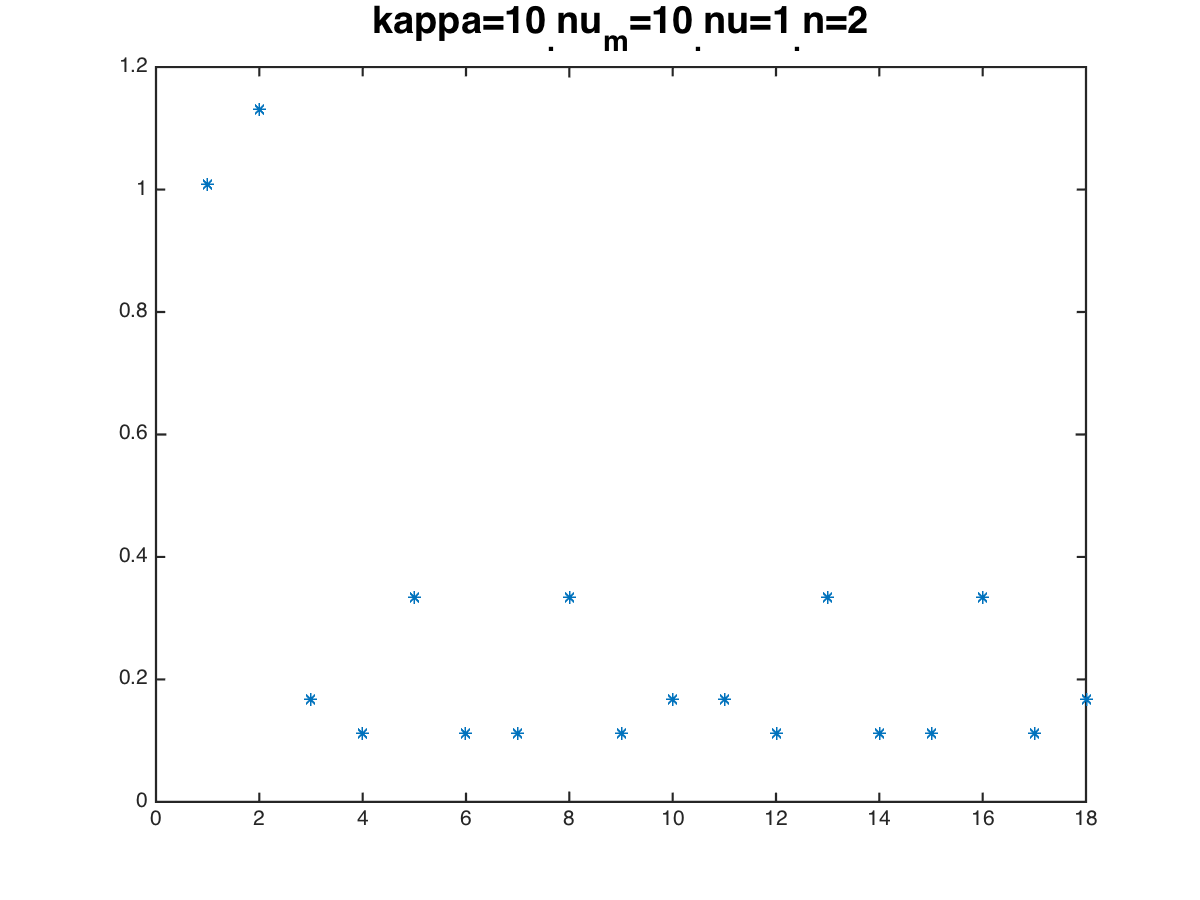
\includegraphics[width=0.5\textwidth]{FLUIDkappa=10_nu_m=10_nu=1_n=2}&
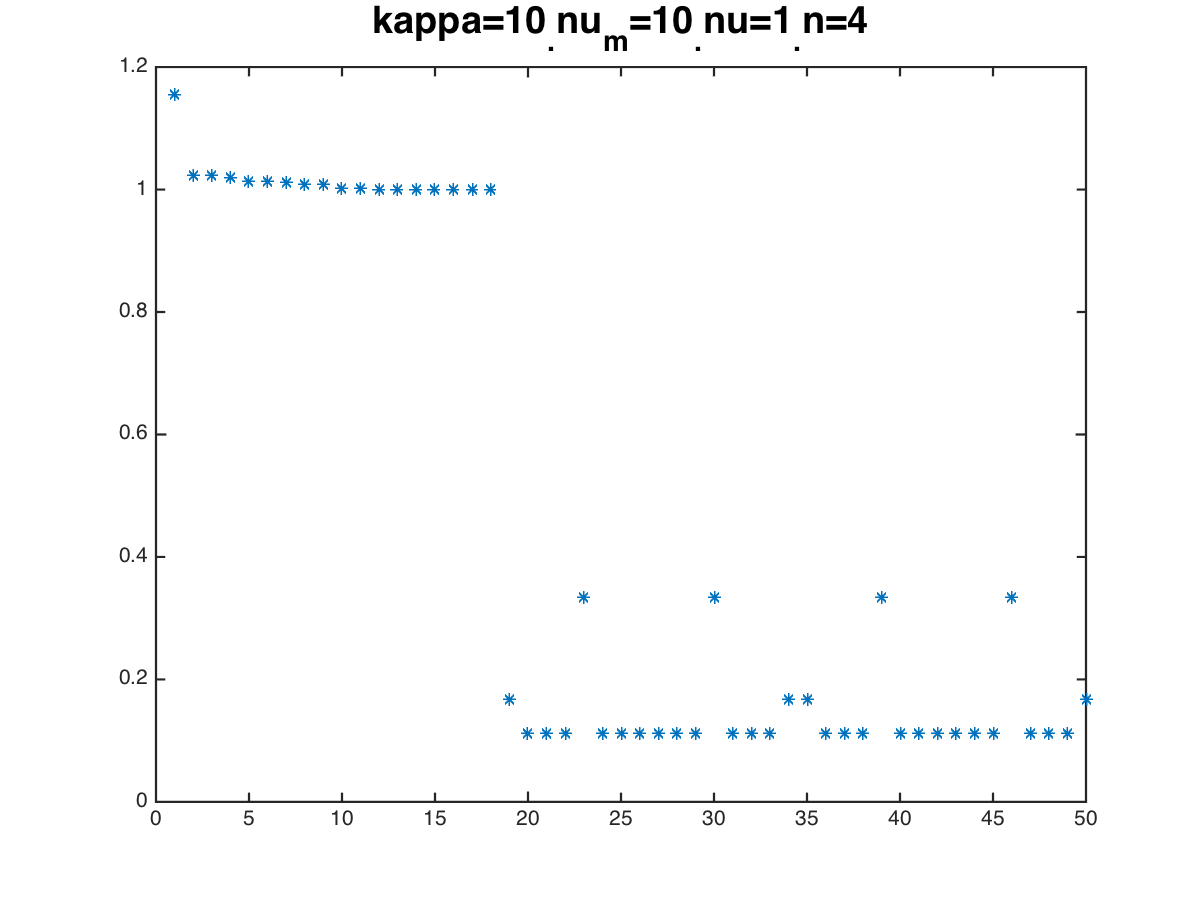
\includegraphics[width=0.5\textwidth]{FLUIDkappa=10_nu_m=10_nu=1_n=4}\\
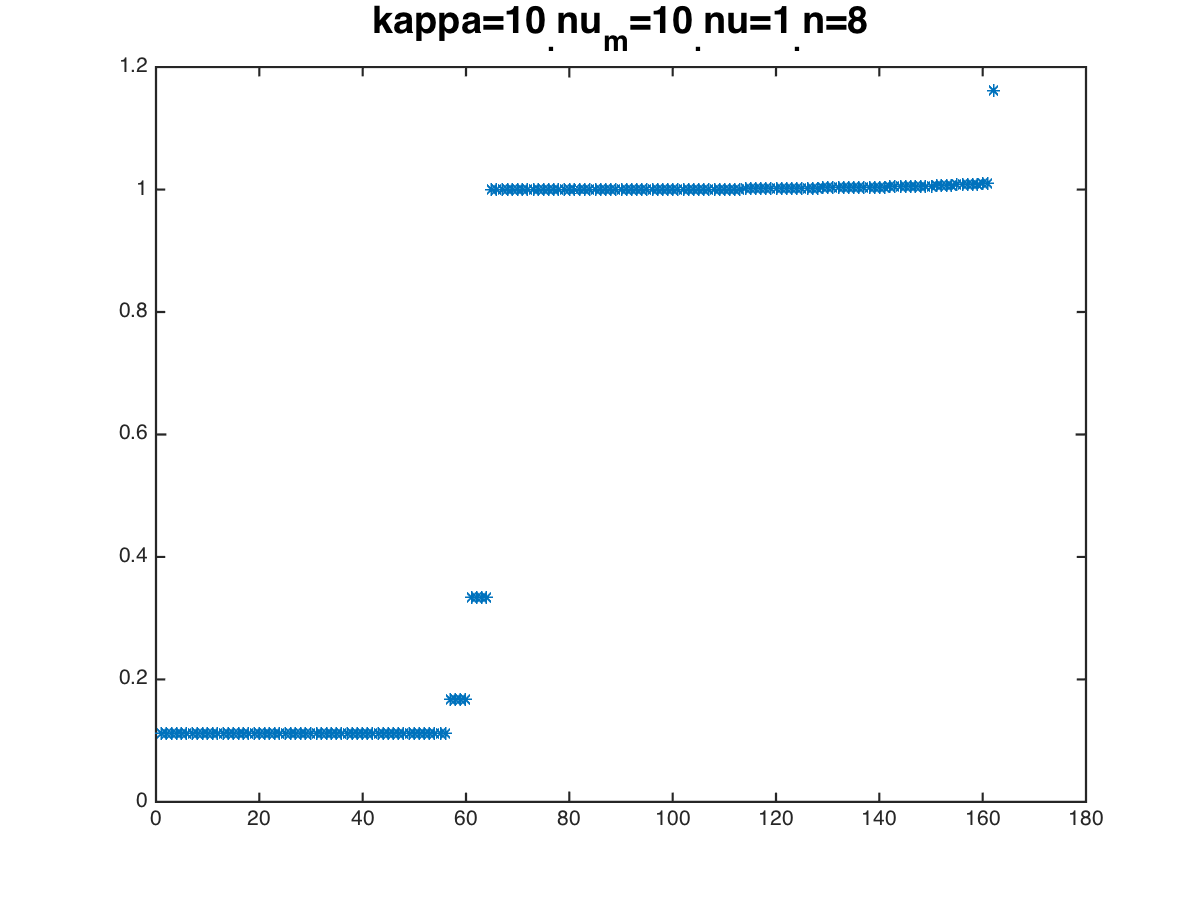
\includegraphics[width=0.5\textwidth]{FLUIDkappa=10_nu_m=10_nu=1_n=8}&
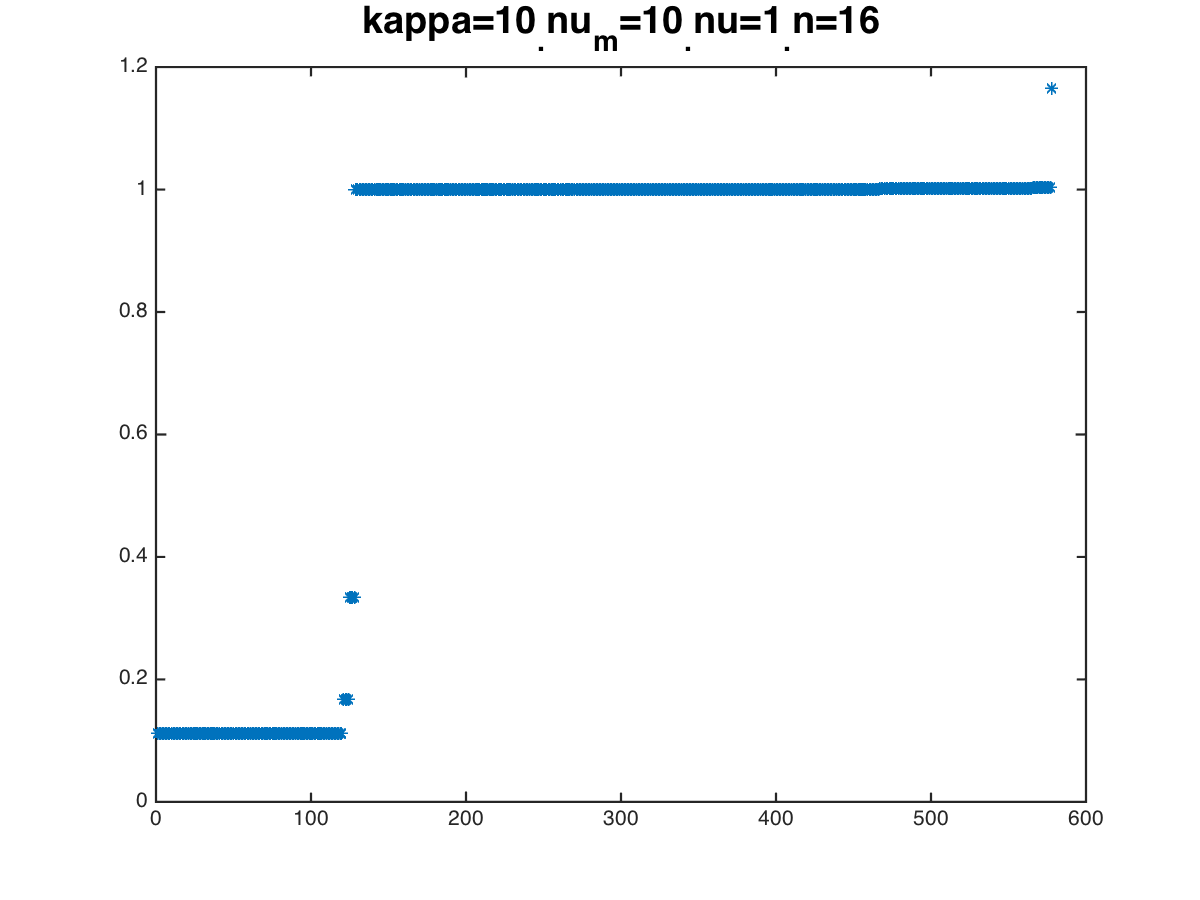
\includegraphics[width=0.5\textwidth]{FLUIDkappa=10_nu_m=10_nu=1_n=16}
\end{array}$
\end{center}
\caption{Eigenvalue plot for various values of n}
\label{pics:blablabla}
\end{figure}
\begin{figure}[h]
\begin{center}$
\begin{array}{cc}
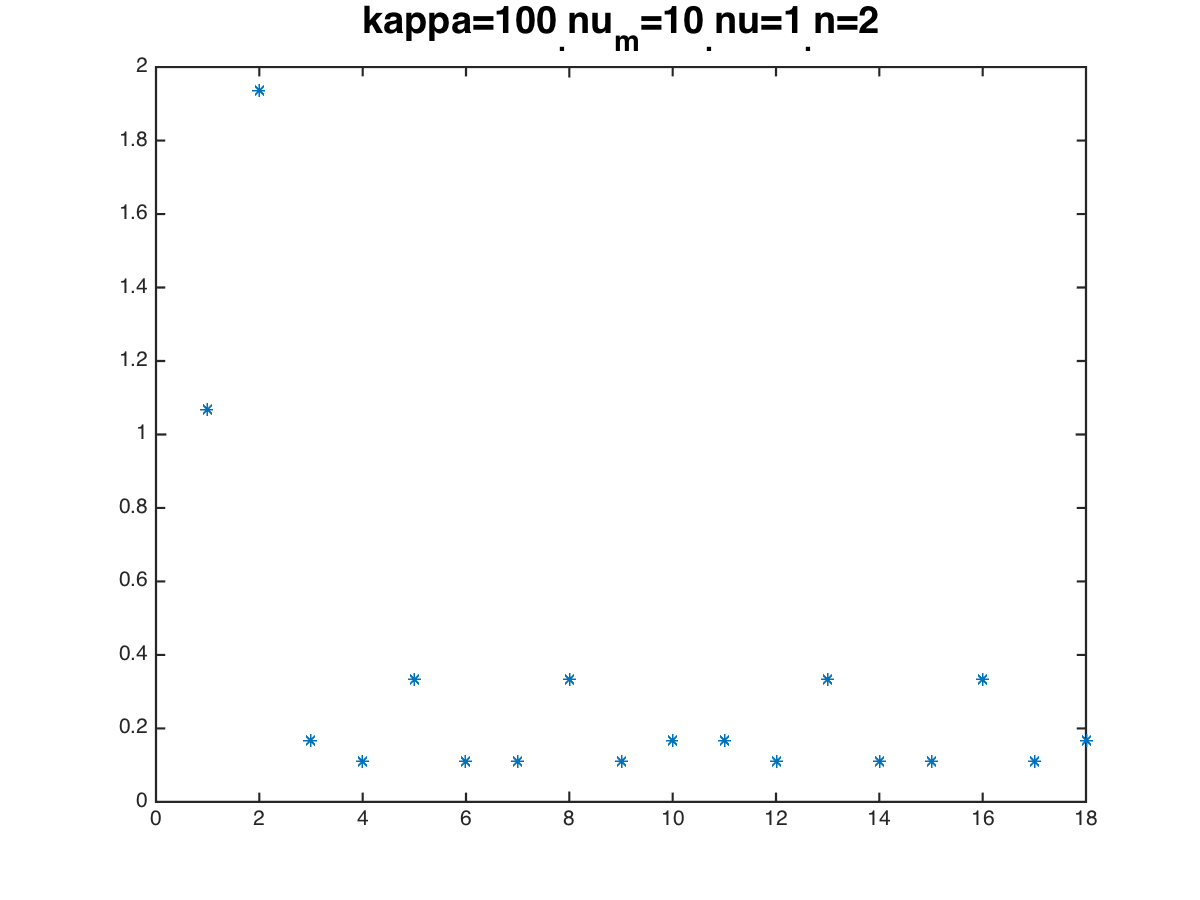
\includegraphics[width=0.5\textwidth]{FLUIDkappa=100_nu_m=10_nu=1_n=2}&
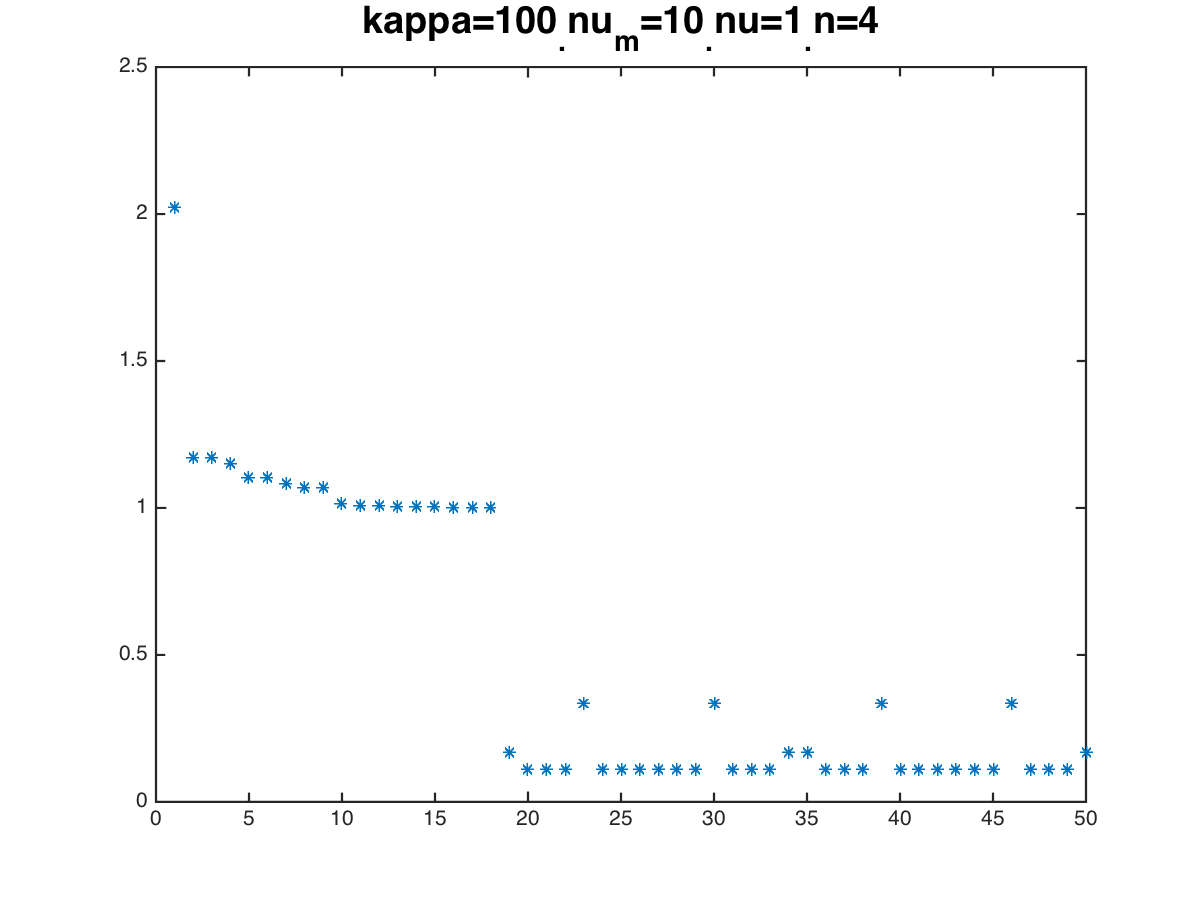
\includegraphics[width=0.5\textwidth]{FLUIDkappa=100_nu_m=10_nu=1_n=4}\\
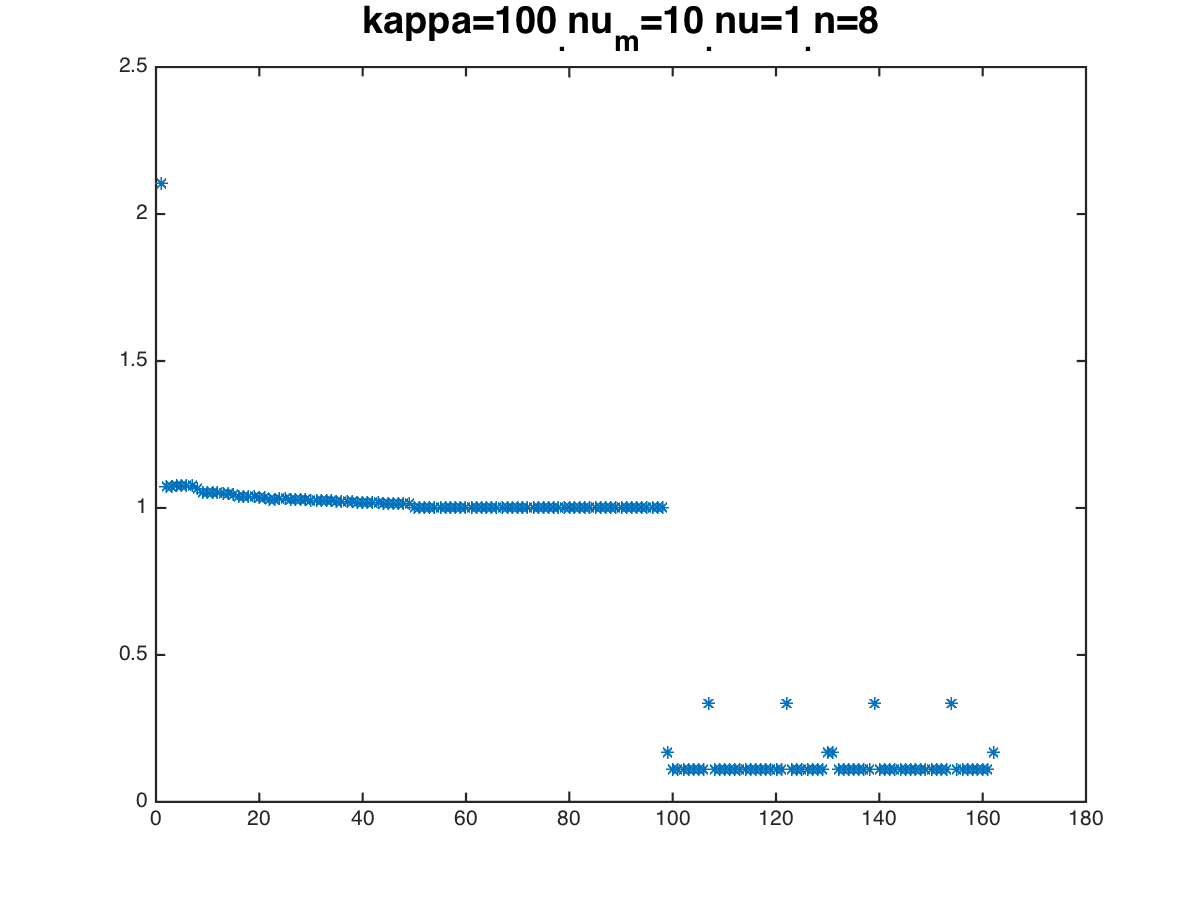
\includegraphics[width=0.5\textwidth]{FLUIDkappa=100_nu_m=10_nu=1_n=8}&
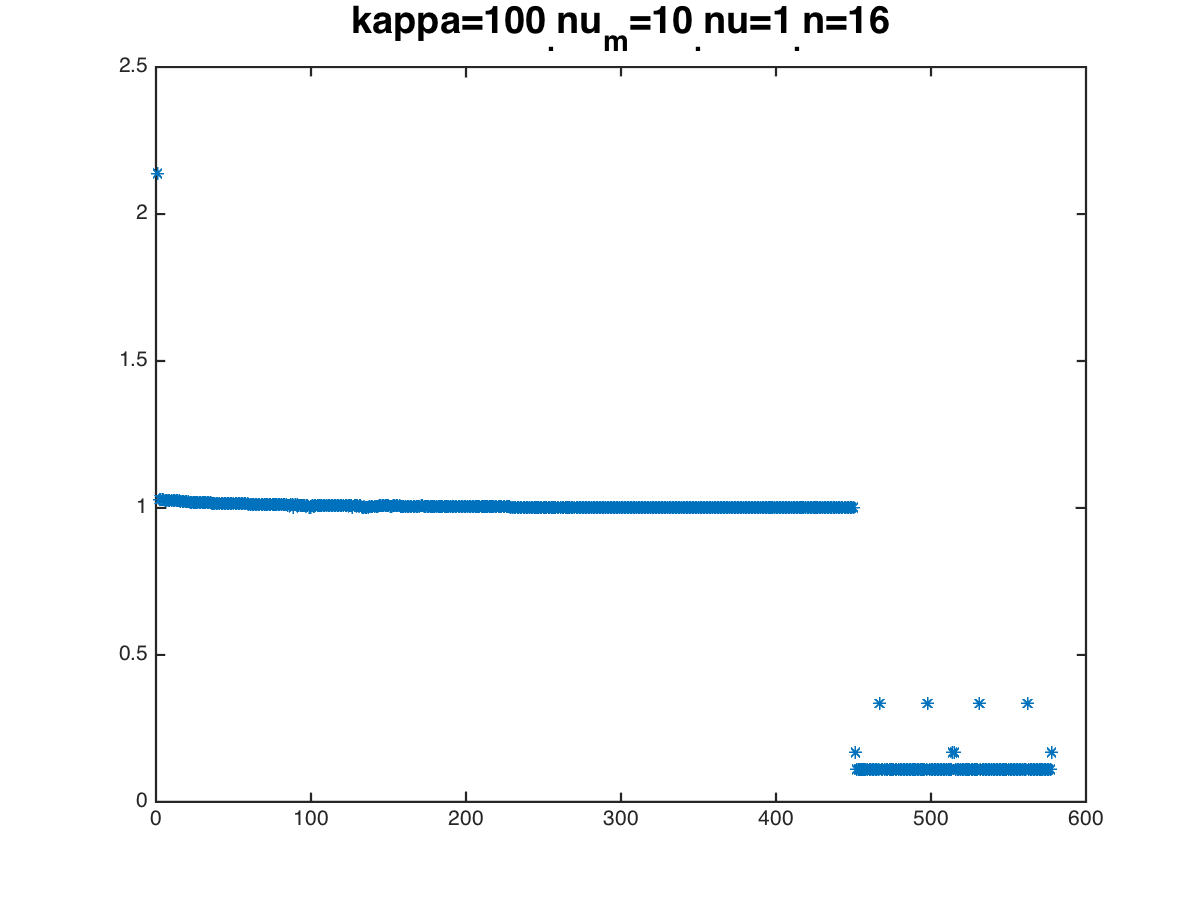
\includegraphics[width=0.5\textwidth]{FLUIDkappa=100_nu_m=10_nu=1_n=16}
\end{array}$
\end{center}
\caption{Eigenvalue plot for various values of n}
\label{pics:blablabla}
\end{figure}

\newpage
\section{Approximating $M+X+CF^{-1}C^T$}


Using the result in [Elman,....] we approximate 
\begin{equation} \label{eq:magnetic}
A = M+X+CF^{-1}C^T \approx M+X+X_s=B,
\end{equation}
were $X_s$ is a scaled vector mass matrix. Solving the generalised eigenvalue
problem
$$Bx = \lambda Ax,$$
produces the following eigenvalue plots.
\begin{figure}[h]
\begin{center}$
\begin{array}{cc}
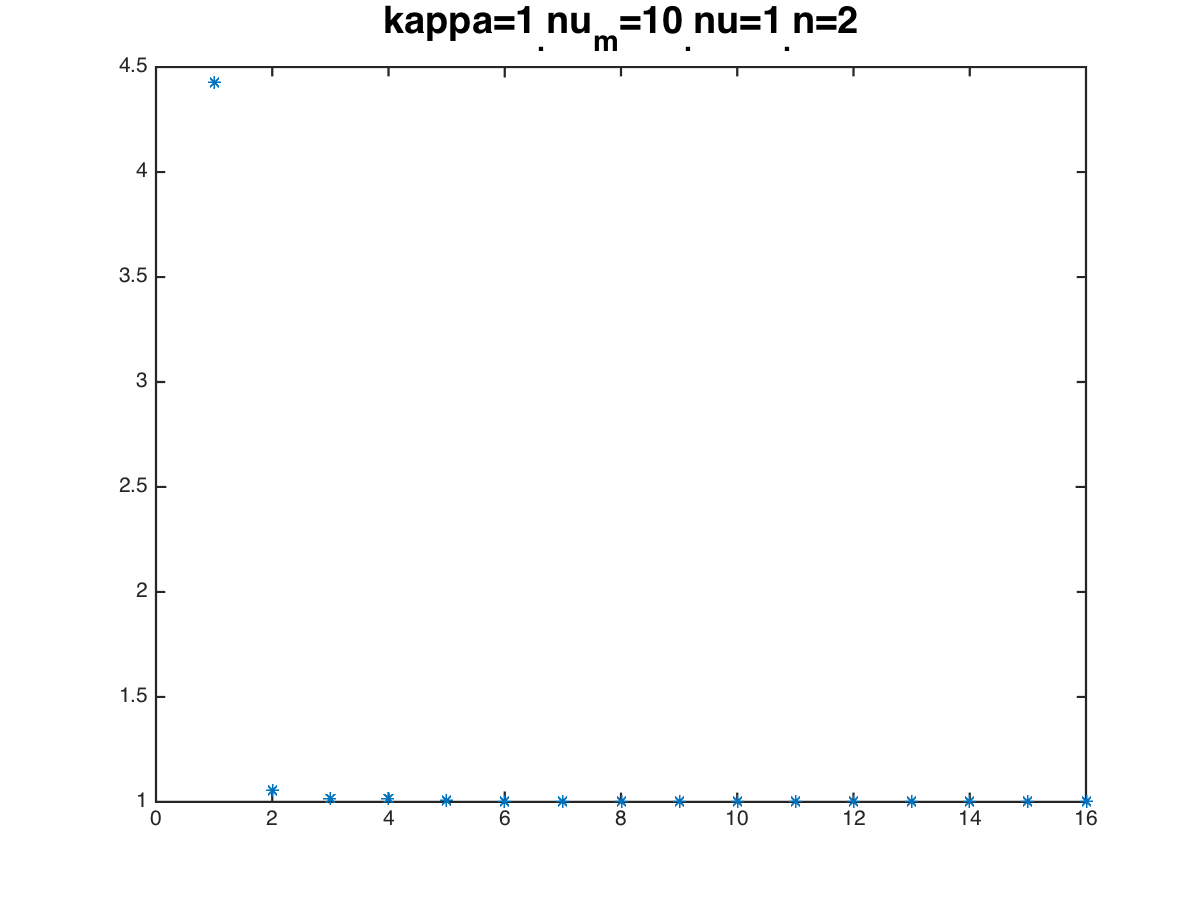
\includegraphics[width=0.5\textwidth]{MAGkappa=1_nu_m=10_nu=1_n=2}&
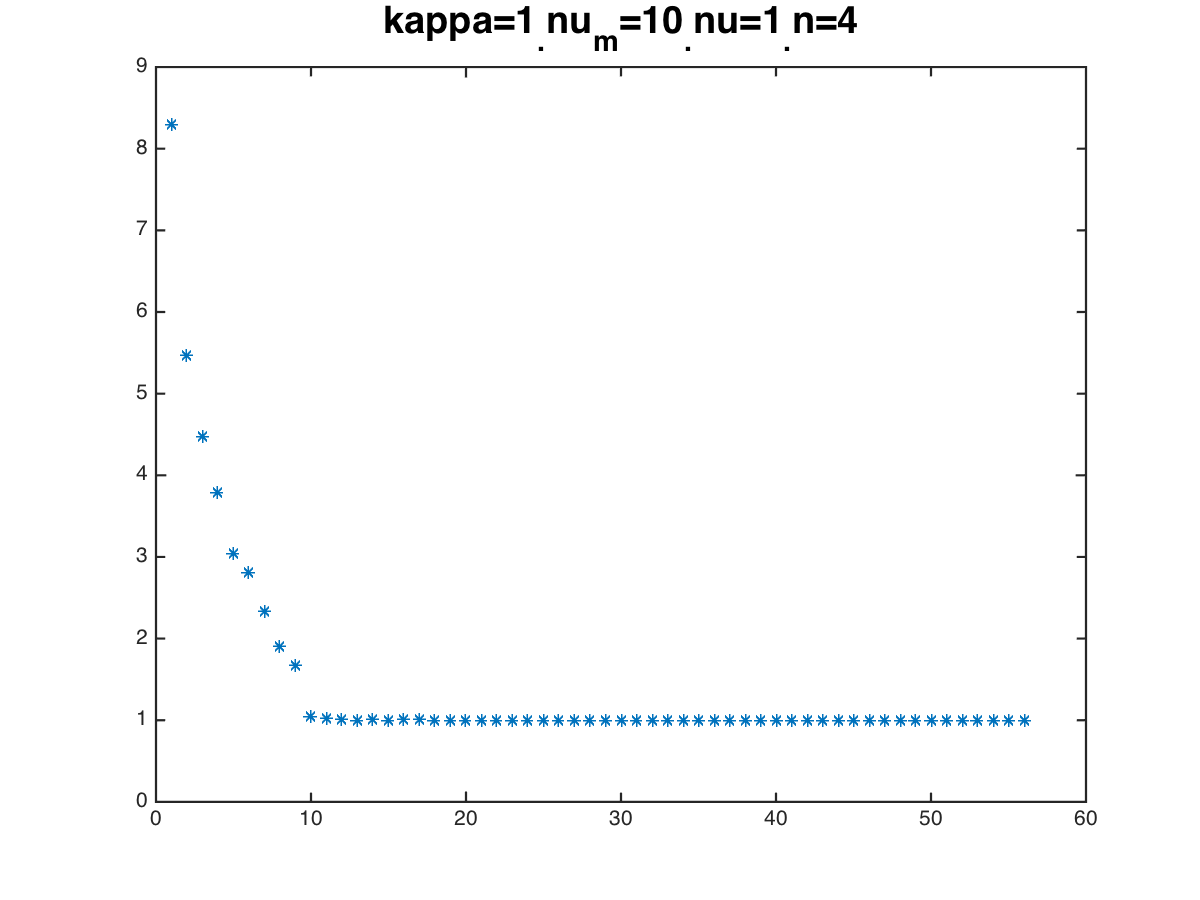
\includegraphics[width=0.5\textwidth]{MAGkappa=1_nu_m=10_nu=1_n=4}\\
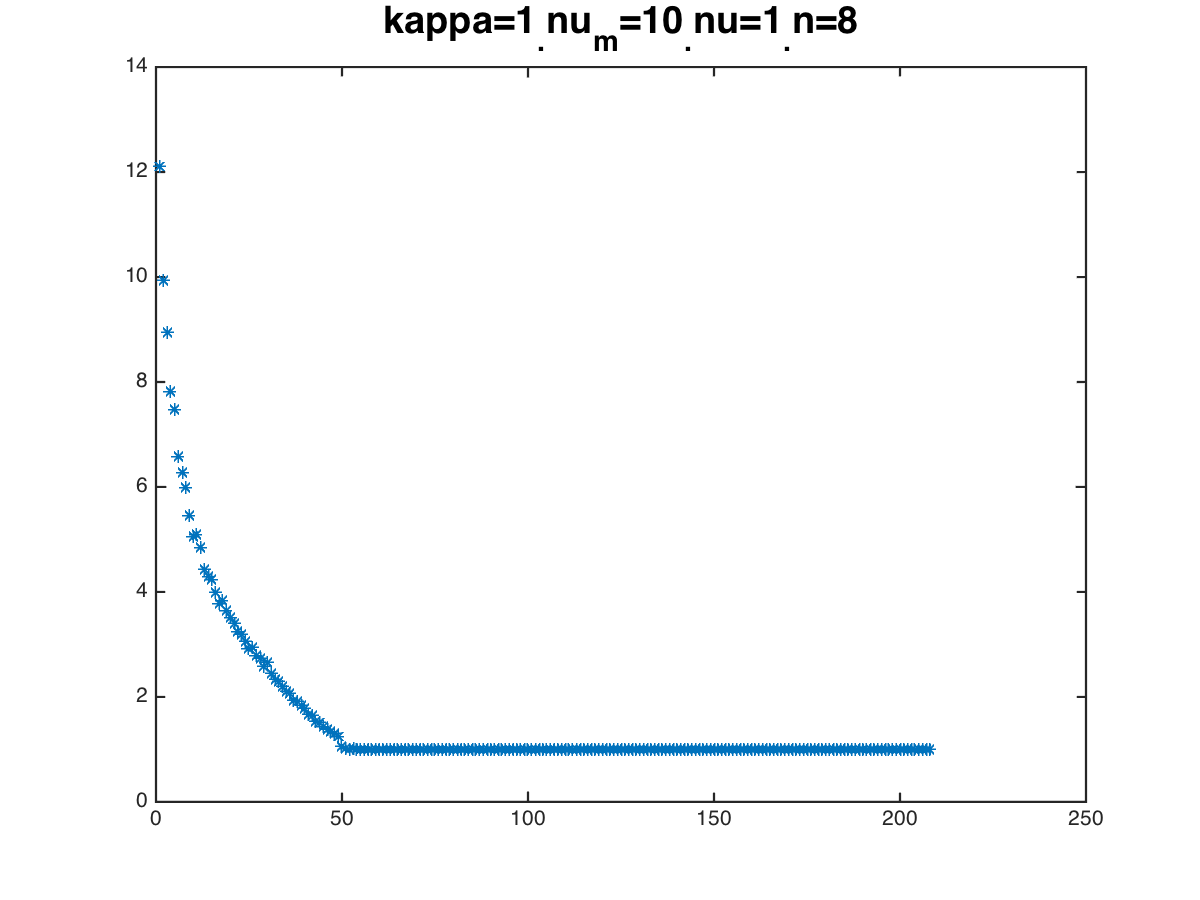
\includegraphics[width=0.5\textwidth]{MAGkappa=1_nu_m=10_nu=1_n=8}&
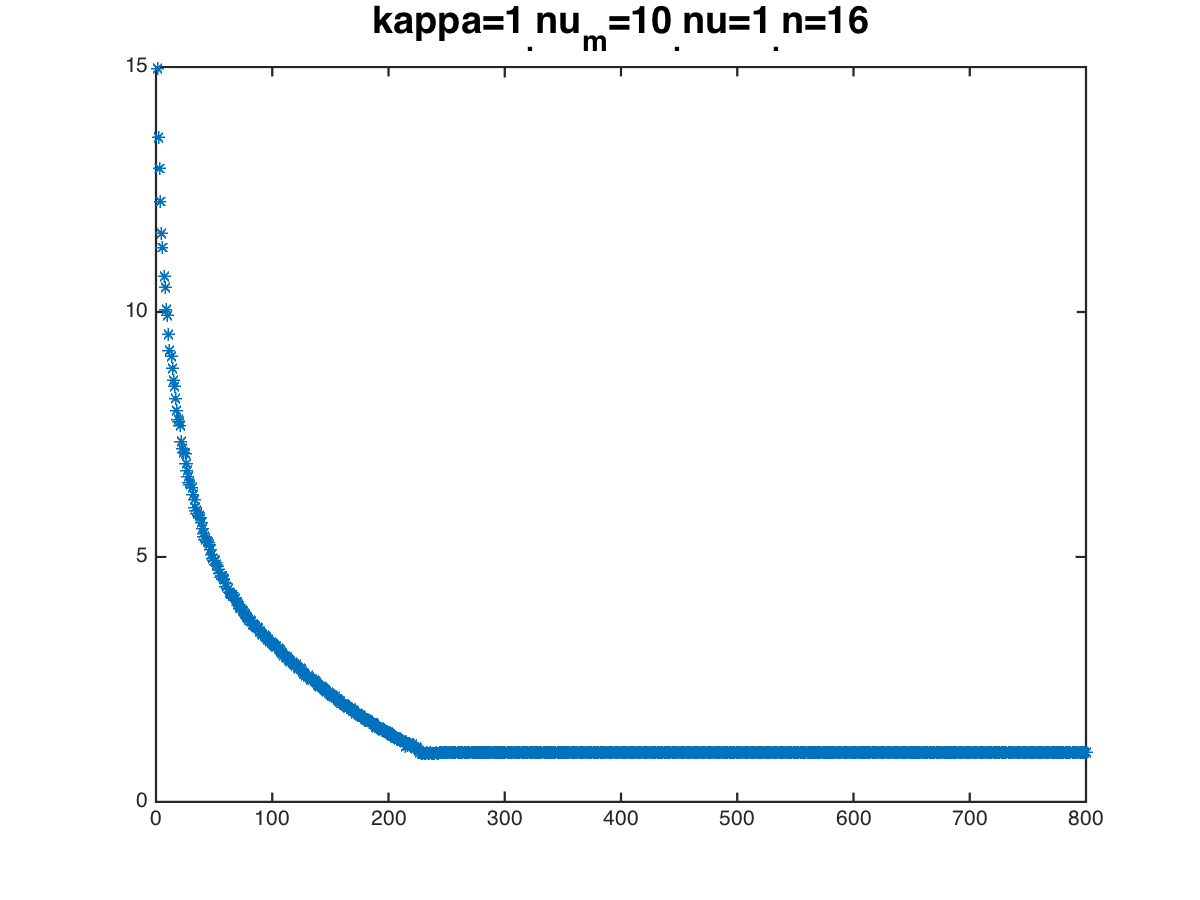
\includegraphics[width=0.5\textwidth]{MAGkappa=1_nu_m=10_nu=1_n=16}
\end{array}$
\end{center}
\caption{Eigenvalue plot for various values of n}
\label{pics:blablabla}
\end{figure}
\begin{figure}[h]
\begin{center}$
\begin{array}{cc}
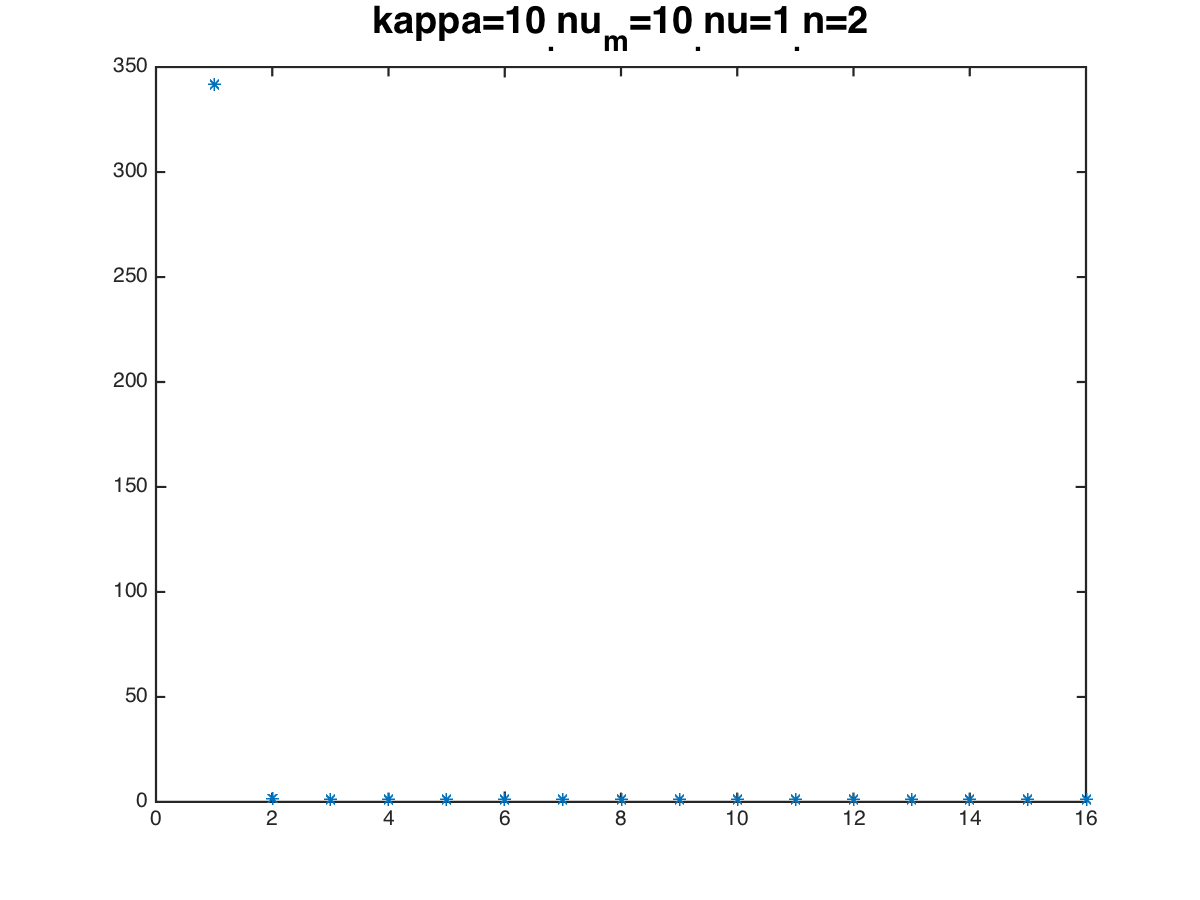
\includegraphics[width=0.5\textwidth]{MAGkappa=10_nu_m=10_nu=1_n=2}&
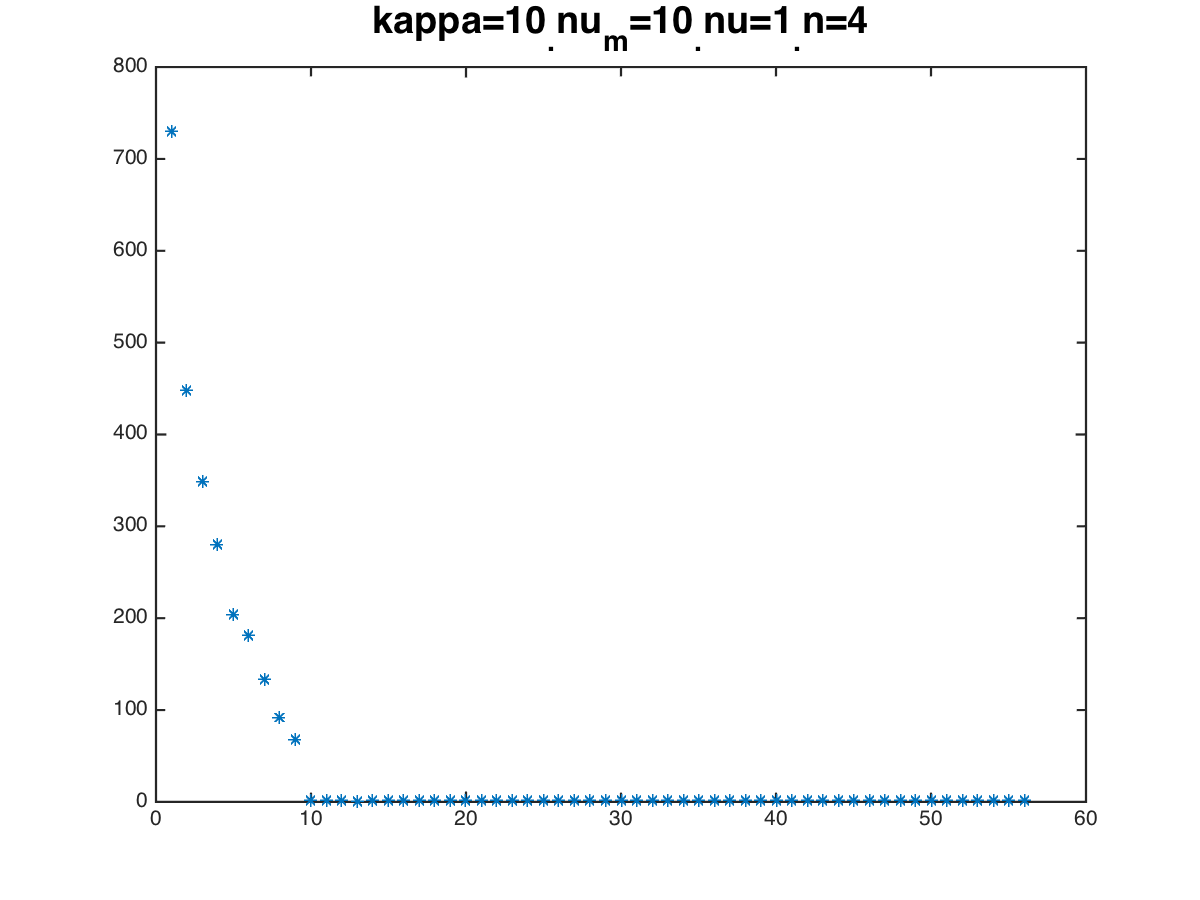
\includegraphics[width=0.5\textwidth]{MAGkappa=10_nu_m=10_nu=1_n=4}\\
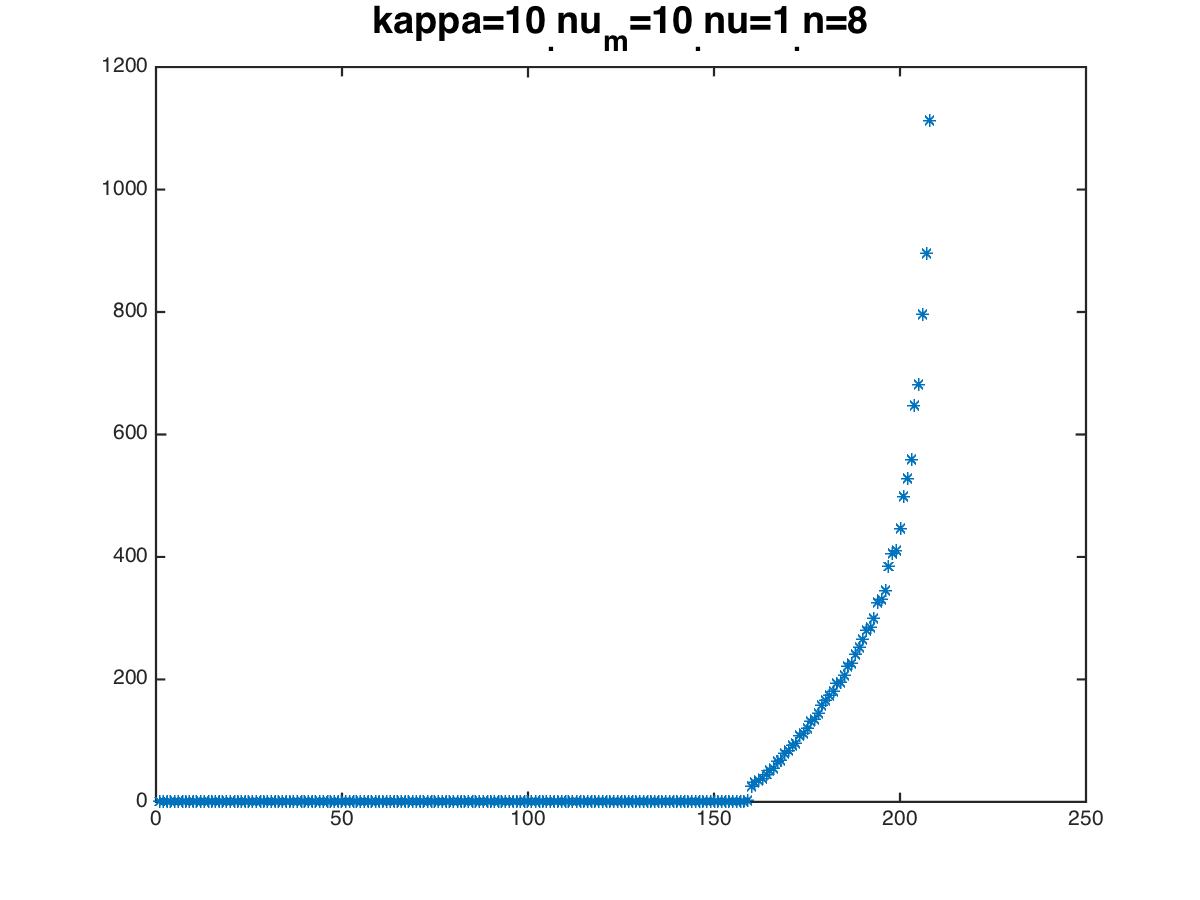
\includegraphics[width=0.5\textwidth]{MAGkappa=10_nu_m=10_nu=1_n=8}&
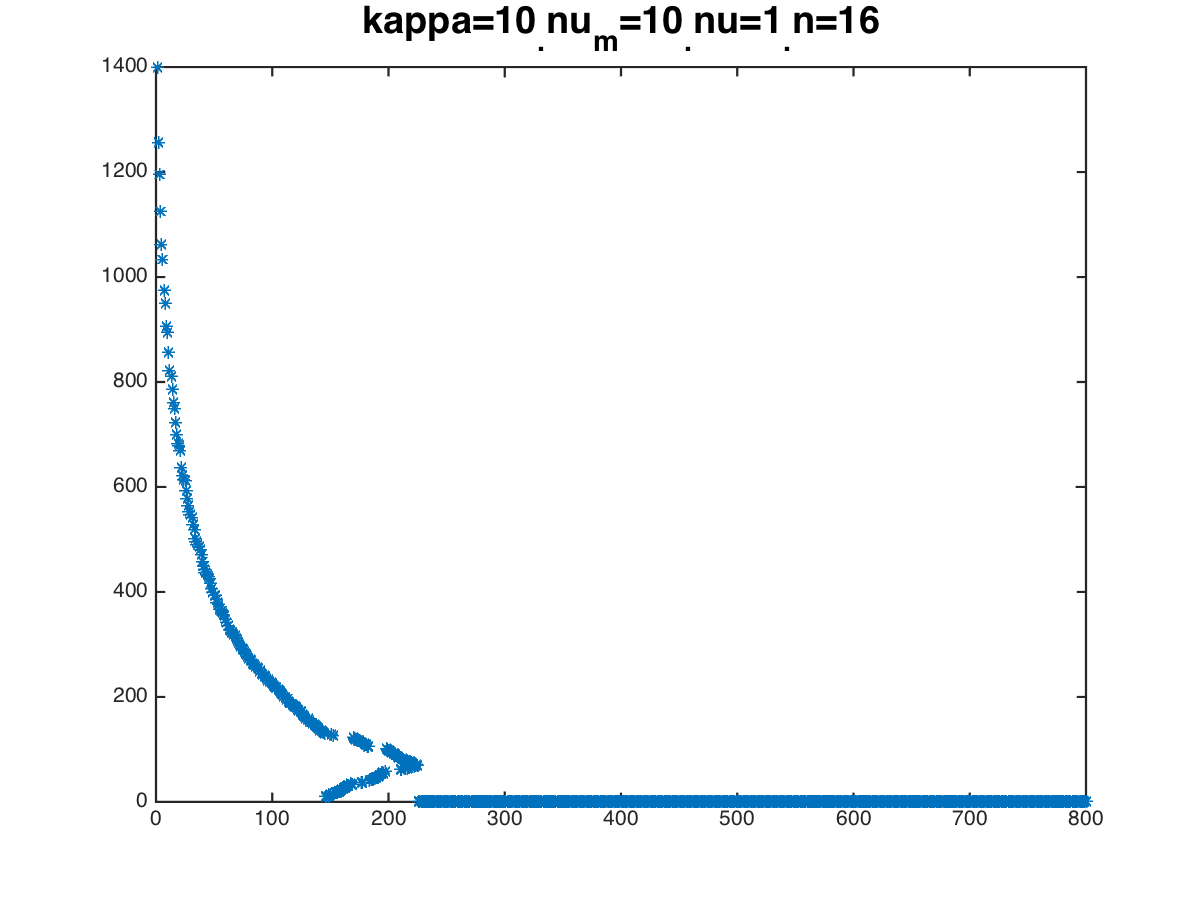
\includegraphics[width=0.5\textwidth]{MAGkappa=10_nu_m=10_nu=1_n=16}
\end{array}$
\end{center}
\caption{Eigenvalue plot for various values of n}
\label{pics:blablabla}
\end{figure}

\section{Discussion}

From the figures, we note that the eigenvalues computed when using the
approximation given in (\ref{eq:magnetic}) seem to spread out as the mesh size,
$n$, gets bigger. However, for the approximation (\ref{eq:fluid}) the eigenvalues seem to be
clustered nicely. There appears to be a single eigenvalue that is about 1.2 for
$\kappa = 10$ and 2 for $\kappa = 100$ that is not clustered. This single
eigenvalue does not, however, seem to increase dramatically as the mesh size
increases. 


\end{document}
